\chapter{ANTECEDENTES / ESTADO DEL \mbox{ARTE}}

\section{Estado del arte}

\subsection{El crecimiento de la analítica de datos en el Internet de las Cosas}

El despliegue masivo de dispositivos conectados ha convertido a la analítica de datos en el elemento central para transformar la telemetría generada por sensores e infraestructuras inteligentes en información accionable. Como señala Y. Liu \cite{liu2025}, el proceso de análisis de datos IoT abarca la recolección, el procesamiento, el almacenamiento y la extracción de conocimiento, y su relevancia se ha extendido a dominios tan diversos como la salud, las ciudades inteligentes, la automatización industrial, el monitoreo ambiental y el transporte inteligente. El crecimiento exponencial del volumen, la velocidad y la variedad de los datos generados por miles de millones de dispositivos ha superado la capacidad de los enfoques de procesamiento tradicionales orientados a lotes, obligando a la creación y adopción de arquitecturas capaces de ingerir, procesar y almacenar flujos continuos de datos en tiempo real (Y. Liu \cite{liu2025}).

Esta transición no es meramente tecnológica: el cambio de paradigma también implica que el valor de los datos IoT depende de la latencia con la que se procesan. Por ejemplo, los datos de temperatura de un motor industrial, pierden gran parte de su utilidad si se analizan horas después de haberse generado, cuando la ventana de acción preventiva ya se ha cerrado. Este factor motiva la centralidad que ha adquirido el procesamiento por flujos (\textit{stream processing}) frente al procesamiento por lotes clásico para los pipelines IoT modernos.

\subsection{Categorización de la analítica de datos IoT}

Y. Liu \cite{liu2025} propone un marco de clasificación que resulta útil para situar cualquier pipeline IoT dentro del panorama general de la disciplina. Este marco de clasificación distingue tres dimensiones complementarias, tal como se muestra en la Figura~\ref{fig:liu2025}:

\begin{itemize}
    \item \textbf{Categorías de análisis}, según el momento y el propósito del procesamiento: análisis descriptivo (qué ha ocurrido), análisis en tiempo real (qué está ocurriendo), análisis predictivo (qué es probable que ocurra) y análisis prescriptivo (qué se debería hacer al respecto).
    \item \textbf{Enfoques de despliegue}: procesamiento centralizado en la nube (\textit{cloud-based}), procesamiento en el extremo de la red (\textit{edge}) y procesamiento intermedio (\textit{fog computing}), cada uno con distintos compromisos entre latencia, ancho de banda y capacidad de cómputo disponible.
    \item \textbf{Componentes funcionales}: ingesta y recolección de datos, almacenamiento y gestión, preprocesamiento y transformación, y finalmente analítica y aprendizaje automático.
\end{itemize}

\begin{figure}[H]
    \centering
    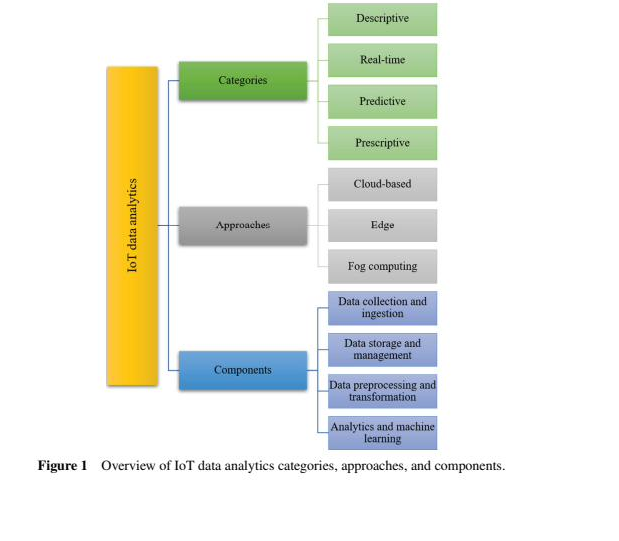
\includegraphics[width=0.75\textwidth]{imagenes/liu2025_fig1.png}
    \caption[Categorías, enfoques y componentes de la analítica de datos IoT]{Categorías, enfoques y componentes de la analítica de datos IoT. Reproducida de Y. Liu \cite{liu2025}, distribuida bajo licencia Creative Commons (CC BY).}
    \label{fig:liu2025}
\end{figure}

\subsection{Arquitecturas de referencia: Lambda y Kappa}

En la literatura sobre procesamiento de grandes volúmenes de datos en streaming destacan dos patrones arquitectónicos ampliamente documentados. La arquitectura Lambda fue propuesta originalmente por N. Marz \cite{marz2011} en 2011, y posteriormente detallada junto con J. Warren \cite{marzwarren2015}; combina una capa de procesamiento por lotes (que recalcula vistas precisas sobre el histórico completo) con una capa de velocidad (que ofrece vistas aproximadas de baja latencia sobre los datos recientes), fusionadas después en una capa de servicio.

\begin{figure}[H]
    \centering
    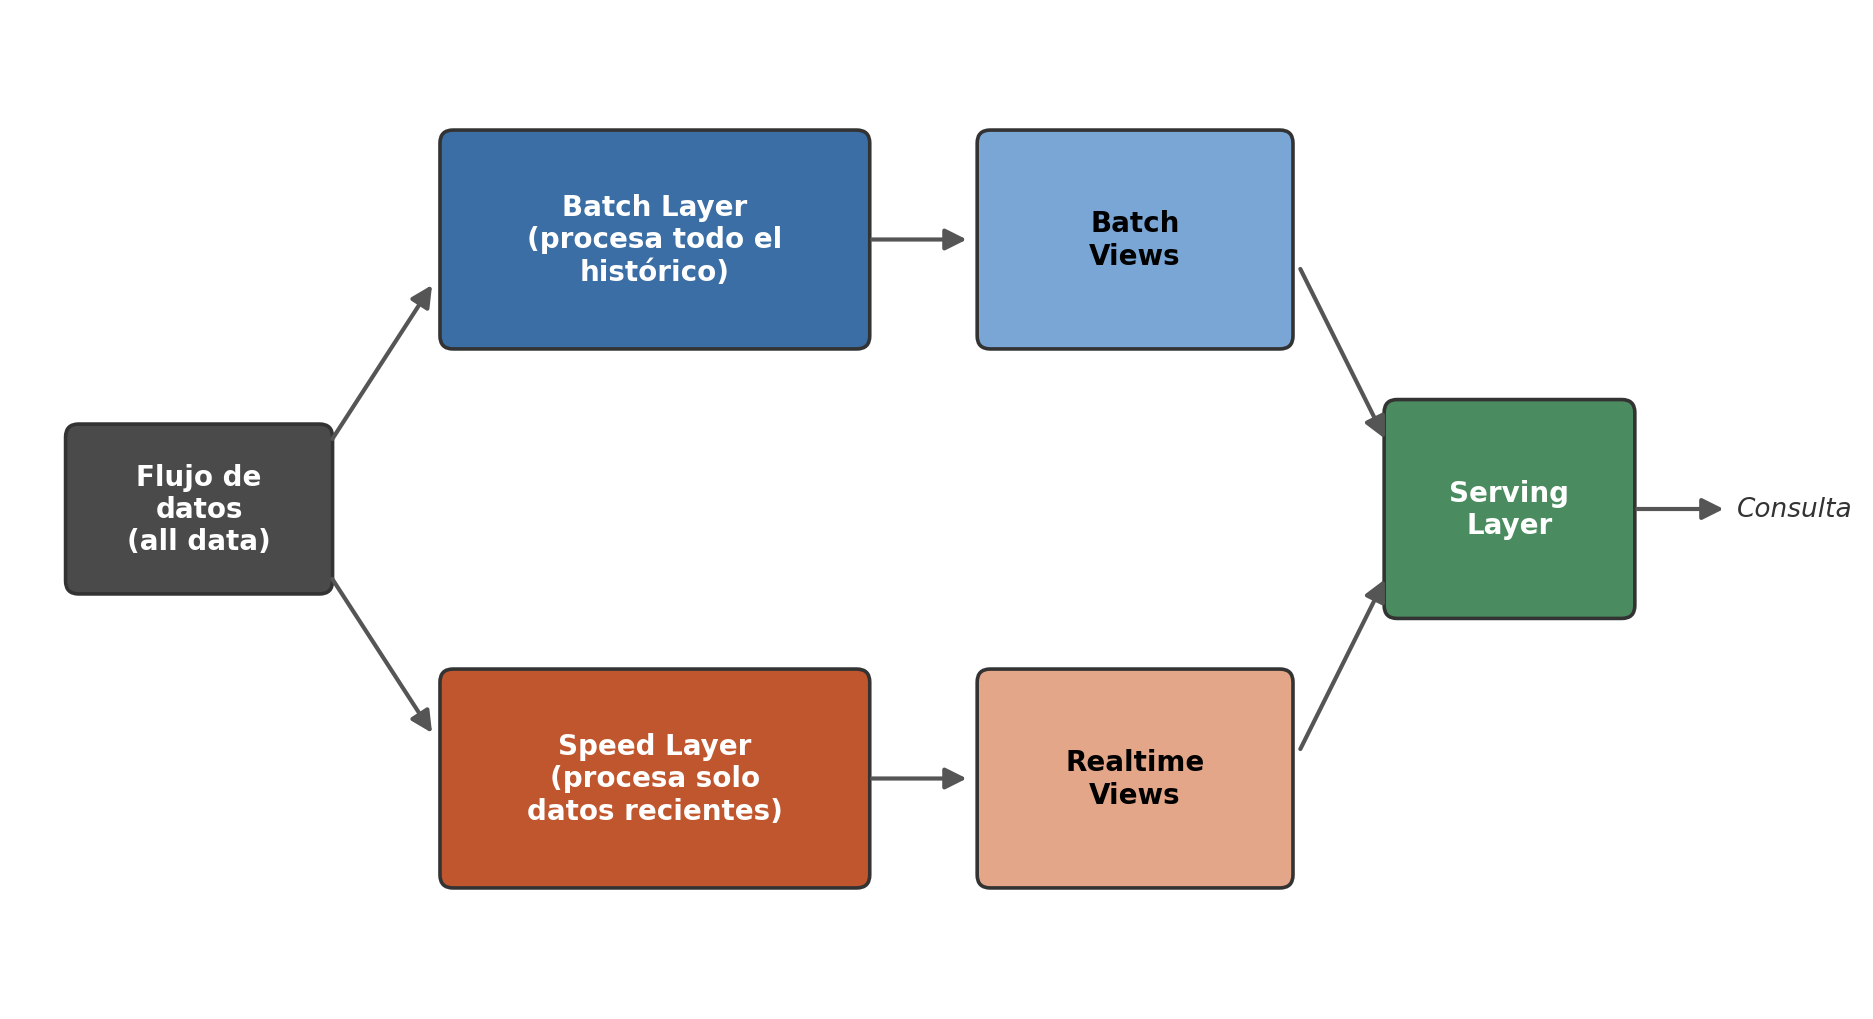
\includegraphics[width=0.8\textwidth]{imagenes/lambda_architecture.png}
    \caption[Arquitectura Lambda]{Arquitectura Lambda: las capas batch y speed se fusionan en la capa de servicio. Elaboración propia a partir de \cite{marz2011} y \cite{marzwarren2015}.}
    \label{fig:lambda}
\end{figure}

Aunque este patrón fue ampliamente adoptado, J. Kreps \cite{kreps2014} señala que exige implementar y mantener la misma lógica de transformación por duplicado (una vez en el sistema batch y otra en el de streaming), y sincronizar ambas versiones resulta muy costoso operativamente. H. Cao y M. Wachowicz \cite{caowachowicz2019} añaden que, además, su dependencia de infraestructura de cómputo intensivo la hace poco adecuada para muchos escenarios IoT.

Como alternativa, J. Kreps \cite{kreps2014} propuso en 2014 la arquitectura Kappa, que elimina la capa de lotes y utiliza un flujo reproducible (\textit{replayable stream}) como fuente única de verdad, de modo que el reprocesamiento histórico se realiza reproduciendo el propio flujo a través del mismo trabajo de streaming.

\begin{figure}[H]
    \centering
    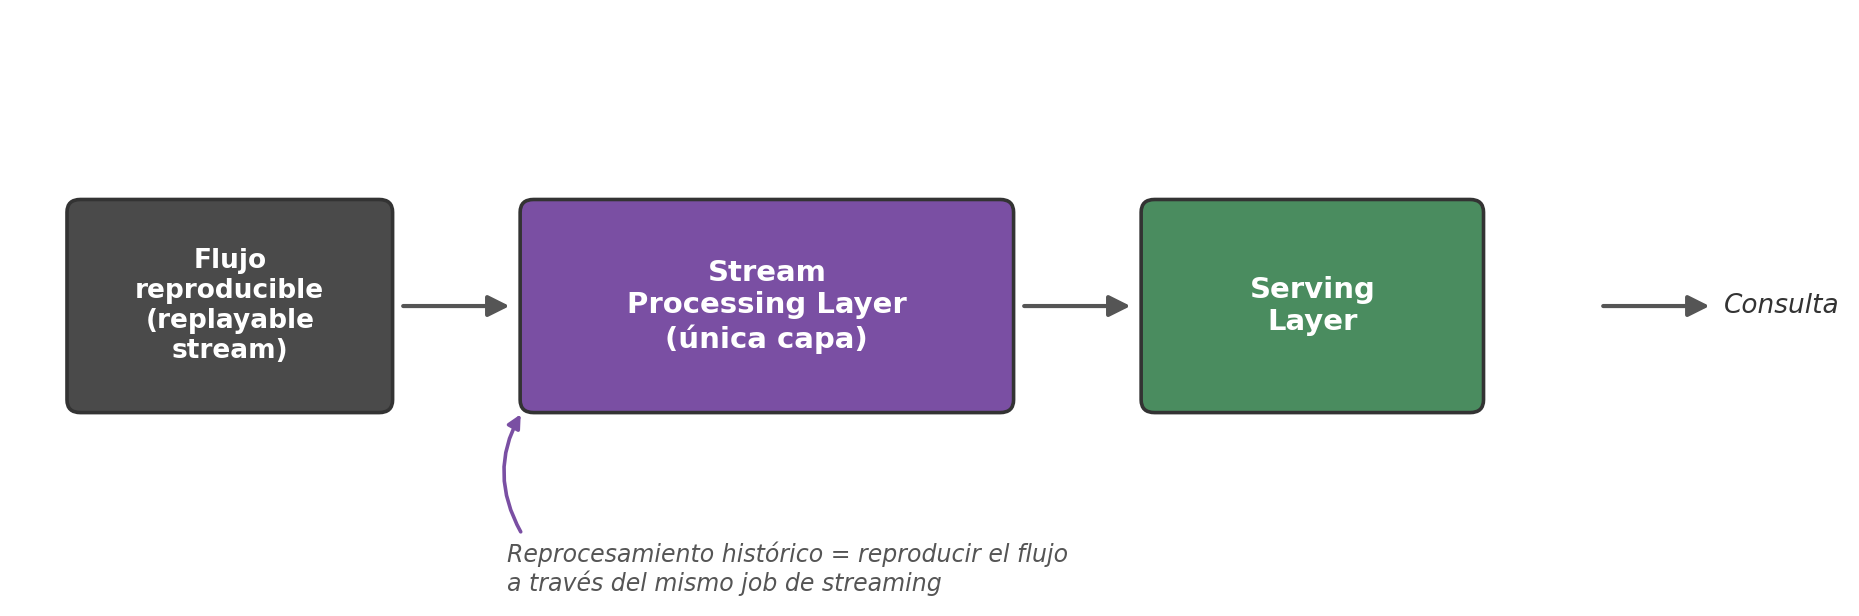
\includegraphics[width=0.85\textwidth]{imagenes/kappa_architecture.png}
    \caption[Arquitectura Kappa]{Arquitectura Kappa: una única capa de procesamiento de streaming, con reprocesamiento histórico mediante reproducción del flujo. Elaboración propia a partir de \cite{kreps2014}.}
    \label{fig:kappa}
\end{figure}

Ejemplos recientes de implementación práctica de Kappa en contextos IoT incluyen a S. Shinde \cite{shinde2025}, quien construye un pipeline de monitorización de temperatura y detección de anomalías con Kafka, Spark Streaming y Streamlit, y a G. Zefkilis \cite{zefkilis2025}, que documenta una variante con Kafka, Spark Streaming, StarRocks y MinIO sobre Docker. Cabe señalar, no obstante, que ambos son tutoriales técnicos de un único autor.

\subsection{Ecosistema de herramientas de código abierto para el procesamiento de datos IoT}

El ecosistema de herramientas de código abierto disponible para cada etapa del pipeline IoT ha madurado considerablemente, como ilustran las implementaciones de S. Shinde \cite{shinde2025} y G. Zefkilis \cite{zefkilis2025} comentadas en la sección anterior. En la etapa de ingesta, los protocolos ligeros de publicación-suscripción como MQTT conviven con brokers que ofrecen puentes nativos hacia sistemas de mensajería distribuida como Apache Kafka, permitiendo desacoplar la capa de dispositivos de la capa de procesamiento. En la etapa de procesamiento de flujos, Apache Flink se ha consolidado como la opción de referencia para el cómputo continuo con semántica de eventos, mientras que Kafka Streams ocupa un nicho más acotado como librería embebida para aplicaciones Java/Scala nativas de Kafka que no requieren un clúster de procesamiento independiente. Apache Spark Structured Streaming, por su parte, se ha consolidado como el estándar de facto de la industria para el procesamiento por micro-lotes, apoyado en la amplitud de su ecosistema y en la unificación del modelo de procesamiento batch/streaming bajo una misma API \cite{lakshmipathy2025}. Para el almacenamiento de series temporales, motores especializados como InfluxDB, TimescaleDB y QuestDB compiten por ofrecer el mejor equilibrio entre velocidad de escritura, compresión y capacidad de consulta analítica; conviene advertir, sin embargo, que buena parte de los benchmarks de rendimiento publicados en este espacio provienen directamente de los fabricantes de cada producto, por lo que deben interpretarse con cautela hasta que exista replicación independiente. Finalmente, en la capa de visualización, Grafana se ha convertido en el estándar de facto para paneles operacionales sobre datos de series temporales, en muchos casos combinado con Prometheus para monitoreo de infraestructura.

T. Domínguez-Bolaño et al. \cite{dominguez2022} complementan esta panorámica con un análisis comparativo de plataformas IoT de código abierto de propósito más general (como ThingsBoard o Eclipse Ditto) que integran varias de estas capas en un único producto, frente al enfoque modular de ensamblar componentes especializados por etapa que caracteriza a los pipelines construidos a medida. Ambos enfoques (plataforma integrada frente a ensamblaje modular de componentes) representan compromisos distintos entre rapidez de despliegue y flexibilidad de adaptación a requisitos específicos de un proyecto.

\subsection{Retos abiertos: seguridad, interoperabilidad y escalabilidad}

Pese a la madurez alcanzada por las herramientas disponibles, Y. Liu \cite{liu2025} y T. Domínguez-Bolaño et al. \cite{dominguez2022} coinciden en señalar tres retos que permanecen abiertos. En primer lugar, la seguridad: la superficie de ataque se amplía con cada dispositivo conectado, muchos de los cuales presentan capacidades de cómputo limitadas que dificultan la implementación de mecanismos de cifrado y autenticación robustos \cite{liu2025}. En segundo lugar, la interoperabilidad: la coexistencia de múltiples protocolos, formatos de datos y estándares de facto entre fabricantes sigue dificultando la integración de dispositivos heterogéneos dentro de una misma plataforma \cite{dominguez2022}. En tercer lugar, la escalabilidad operativa: ejecutar y mantener en producción los distintos componentes distribuidos que conforman la pila (el broker de mensajería, el motor de procesamiento de streaming y el orquestador de contenedores) exige un nivel de especialización que no siempre está disponible en equipos de tamaño reducido \cite{liu2025}.

En conjunto, la evidencia revisada sugiere que las herramientas de código abierto para el procesamiento de datos IoT son hoy suficientemente maduras para competir con las ofertas propietarias en la nube en la mayoría de los casos de uso, a costa de una mayor carga operativa que exige experiencia técnica para configurar, escalar y asegurar cada componente del pipeline.

\section{Análisis de alternativas y criterios de selección}

La elección de un motor concreto para la etapa de procesamiento de flujos dentro de una arquitectura Kappa no admite una respuesta universal: distintos motores optimizan para distintos compromisos, y la decisión debe fundamentarse en criterios explícitos aplicables a cualquier proyecto de procesamiento de telemetría IoT, no en preferencias de herramienta. A continuación se plantean los criterios considerados y su aplicación al dominio de la telemetría IoT industrial en general.

\begin{itemize}
    \item \textbf{Alineación latencia-requisitos vs. cadencia de generación de datos}: si la frecuencia de emisión de los dispositivos es del orden de segundos a decenas de segundos, un motor de procesamiento por micro-lotes no introduce una degradación perceptible; ya que la ganancia de latencia sub-segundo con un motor de streaming nativo solo es relevante cuando el caso de uso exige control reactivo o detección de eventos críticos en tiempo real.
    \item \textbf{Madurez del ecosistema y de las APIs para el lenguaje de implementación}: la profundidad de soporte de un lenguaje concreto (por ejemplo, Python) varía entre motores; un ecosistema con API nativa más madura reduce fricción de desarrollo y mantenimiento.
    \item \textbf{Unificación del modelo de procesamiento batch/streaming}: algunos motores permiten expresar lógica de procesamiento por lotes y en streaming bajo una misma API, lo que simplifica la arquitectura cuando ambos modos de procesamiento coexisten en el sistema.
    \item \textbf{Disponibilidad de talento y curva de adopción}: la disponibilidad de profesionales con experiencia previa en una tecnología concreta condiciona la viabilidad de mantenimiento y escalado de un sistema en producción a largo plazo.
\end{itemize}

En el dominio del procesamiento de telemetría de dispositivos IoT industriales, la cadencia habitual de generación de eventos (típicamente del orden de segundos) sitúa los requisitos de latencia del sistema muy por debajo del umbral en el que las ventajas de un motor de streaming nativo resultan determinantes. En estos escenarios, un motor de procesamiento por micro-lotes con ventanas de agregación temporal ofrece garantías de tolerancia a fallos y semántica \textit{exactly-once} equivalentes a las de un motor de streaming nativo, sin incurrir en complejidades operativas adicionales. Este análisis no descarta la idoneidad de los motores de streaming nativo en escenarios de mantenimiento predictivo con requisitos de control reactivo o detección de eventos críticos en tiempo real, donde la latencia extremo a extremo resulta un factor determinante del diseño.

\section{Contexto y justificación}

El estado del arte revisado en la sección anterior pone de manifiesto un patrón recurrente: la mayor parte de las referencias sobre arquitecturas Kappa para IoT disponibles hoy (tutoriales de ingeniería, publicaciones de blog técnico, documentación de proyectos open-source) tienen un carácter fundamentalmente demostrativo. Su objetivo es ilustrar un concepto (por ejemplo, monitoreo de temperatura con Kafka, Spark Streaming y Streamlit, o un pipeline equivalente con StarRocks y MinIO), más que ofrecer una implementación completa y reproducible. Esta brecha entre la abundancia de ejemplos ilustrativos y la escasez de implementaciones íntegramente reproducibles constituye la primera motivación de este TFM: construir, documentar y poner a disposición pública un pipeline IoT completo, containerizado y basado exclusivamente en herramientas de código abierto, que sirva tanto como artefacto académico evaluable como referencia técnica reutilizable por terceros.

En segundo lugar, el propio proceso de revisión de la literatura evidenció vacíos concretos que este proyecto puede contribuir a cerrar, al menos parcialmente, desde la práctica: no existe un trabajo independiente que documente el comportamiento de un broker MQTT de perfil ligero en el extremo de la red (\textit{edge tier}) acoplado a un microservicio de bridging dedicado hacia Kafka, un patrón que la bibliografía consultada menciona solo de forma tangencial y sin evaluación propia. La gobernanza de esquemas mediante Avro y un registro como Apicurio sí está documentada como buena práctica en arquitecturas de streaming de propósito general (especialmente en contextos de flotas de dispositivos que evolucionan con el tiempo), pero no aparece integrada como componente explícito en ninguna de las implementaciones Kappa-IoT de código abierto revisadas (\cite{shinde2025}; \cite{zefkilis2025}) ni en los trabajos académicos consultados (\cite{liu2025}; \cite{dominguez2022}; \cite{caowachowicz2019}). Incorporar esta pieza no solo resuelve una necesidad técnica real (evolución controlada del esquema de telemetría a medida que cambian los tipos de sensor o los campos capturados), sino que aporta un elemento diferenciador respecto a los patrones de referencia Kappa-IoT existentes, acercando este pipeline a las prácticas ya consolidadas en arquitecturas de streaming de propósito general.

Finalmente, el diseño de doble sumidero (dual sink: métricas agregadas por ventana temporal hacia TimescaleDB para consumo en Grafana, y eventos individuales enriquecidos hacia PostgreSQL para consumo analítico) responde a una necesidad práctica de separar el consumo operacional en tiempo casi real (monitorización de planta, alertas) del consumo analítico orientado a negocio (reporting, análisis histórico, cruces con otras fuentes corporativas). Este patrón de separación si está documentado en la industria sobre servicios gestionados propietarios; por ejemplo, el caso de AWS con la flota de vehículos de SOCAR, documentado por DoYeun Kim et al. \cite{kimetal2022}, que combina un camino en tiempo real hacia DynamoDB con un camino por lotes hacia S3/Athena/QuickSight para reporting, pero no aparece como patrón explícito en ninguna de las arquitecturas Kappa de referencia íntegramente open-source revisadas, que suelen asumir un único sumidero de salida.

En conjunto, estos tres elementos (reproducibilidad íntegra en código abierto, gobernanza de esquemas mediante Apicurio/Avro, y separación de sumideros operacional/analítico) justifican la elección de la arquitectura desarrollada en este trabajo no como una simple aplicación de un patrón ya resuelto, sino como una propuesta que extiende el patrón Kappa de referencia en direcciones que la literatura actual documenta de forma incompleta.

\section{Planteamiento del problema}

De la revisión anterior se desprende que, si bien existen múltiples implementaciones ilustrativas de arquitecturas Kappa aplicadas a IoT, y patrones equivalentes de gobernanza de esquemas y doble sumidero documentados en contextos de streaming de propósito general o sobre servicios gestionados propietarios, ninguna implementación Kappa-IoT íntegramente open-source revisada combina simultáneamente: (i) un broker MQTT ligero en el extremo acoplado a un microservicio de bridging dedicado hacia Kafka; (ii) un registro de esquemas Avro que gobierne la evolución del contrato de datos entre la capa de ingesta y la capa de procesamiento; y (iii) una estrategia de doble sumidero que separe explícitamente el consumo operacional en tiempo real del consumo analítico enriquecido. Esta falta no es meramente una cuestión de completitud técnica: sin gobernanza de esquemas, cualquier cambio en el formato de telemetría de los dispositivos (por ejemplo, la incorporación de un nuevo tipo de sensor) obliga a coordinar manualmente cambios en todos los consumidores del flujo, un problema de mantenibilidad que se agrava a medida que crece el número de equipos y sitios monitorizados.

A esto se suma una limitación práctica adicional: la mayoría de los recursos formativos y de referencia disponibles para diseñar este tipo de pipelines dependen, en algún punto de la cadena, de servicios gestionados o plataformas propietarias (colas de mensajería en la nube, motores de streaming como servicio, o plataformas de ingesta IoT gestionadas como AWS IoT Core o Azure IoT Hub), lo que dificulta su adopción en contextos donde se requiere control total sobre el despliegue, ausencia de dependencia de un proveedor concreto, o simplemente la posibilidad de ejecutar el sistema completo en un entorno local o on-premise reproducible mediante contenedores.

En consecuencia, el problema central que este TFM aborda puede formularse como: \textbf{la falta de una implementación de referencia, íntegramente open-source y containerizada, de una arquitectura Kappa para IoT que integre bridging MQTT-Kafka en el edge, gobernanza de esquemas mediante Avro/Apicurio, y una estrategia de doble sumidero que separe el consumo operacional del analítico}. Este TFM propone diseñar, implementar y documentar dicha arquitectura utilizando un conjunto de telemetría energética industrial como caso de estudio, evaluando su viabilidad técnica y dejando como artefacto reutilizable el código, la configuración de despliegue y la documentación asociada.
